\documentclass{article}[18pt]
\usepackage{../../../format}
\lhead{CT}


\begin{document}
\begin{center}
\underline{\huge CT Revision}
\end{center}
\section{What is computer hardware}
Three phases of circuit design:
\begin{itemize}
	\item Functional specification - what the IC is supposed to do
	\item Register transfer level - Design of chips and links
	\item Mapped to physical layout - RTL design made appropriate for silicon
\end{itemize}
NAND gates are functionally complete, as can be shown below
\begin{center}
	\includegraphics[scale=0.5]{"NAND"}
\end{center}
\subsection{Adders}
Half adders and full adders are capable of doing binary arithmetic, the advantage of a full adder is that it can take in a carry, allowing them to be chained to process more bits
\begin{center}
	\includegraphics[scale=0.5]{"full_adder"}
\end{center}
Chaining can work as so, with n bit strings $X_1X_2...X_n$ and $Y_1Y_2...Y_n$
\begin{itemize}
	\item A half adder adds the first bits of each string, output sum
	\item The carry is fed into a full adder, along with the next two bits of each string, output sum
	\item This carry is fed into another full adder, along with the next two bits of each string, output sum
	\item This keeps going until you reach the nth bit, output sum and carry
\end{itemize}
\subsection{Microarchitecture}
Components in a CPU microarchitecture:
\begin{itemize}
	\item Datapath - Data processing operations
	\item Control - Tells everything what to do
	\item Cache - Used to store regularly accessed memory items
\end{itemize}
\subsection{Buses}
Types of buses
\begin{itemize}
	\item Data bus - Contents of memory locations between the processor and main memory
	\item Address Bus - Addresses of locations in main memory
\end{itemize}
\textbf{Bus Width} - Number of parallel wires in a bus\\
The width of a the \textbf{data bus} determines word size\\
The width fo the \textbf{address bus} determines size of addressable memory
\subsection{Processor cycle}
\begin{itemize}
	\item Instruction fetch - Give instruction address, get instruction back
	\item Instruction decode - Interpret the stored instruction
	\item Operand fetch - Give address of required data, get data back
	\item Execute instruction - Perform necessary actions, may include a write back substage
\end{itemize}
\subsection{Layers of abstraction}
\begin{center}
	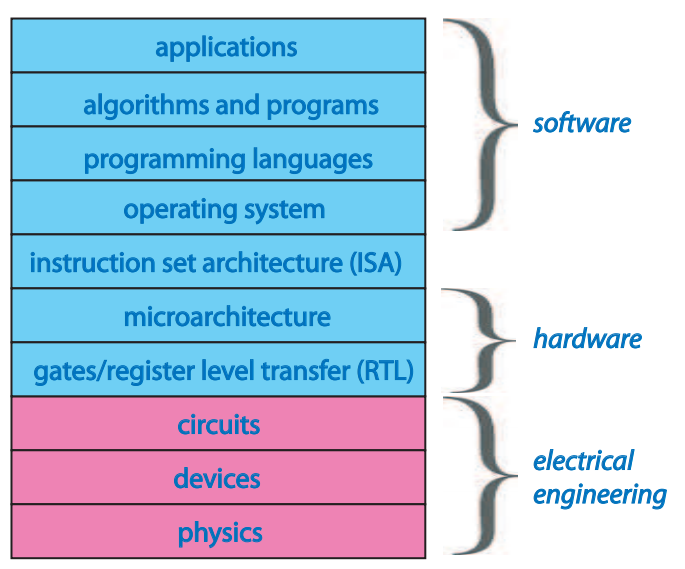
\includegraphics[scale=0.5]{CSys}
\end{center}
\subsection{Processor electronics}
\textbf{Northbridge} - Fast communications amongst critical components\\
\textbf{Southbridge} - Slow communications amongst non critical components (like peripherals)\\
\\
Components of an integrated circuit - Transistors interconnected by microscopic wires\\
\\
The current trend in microprocessor design is to produce multi core processors, which can give better computational improvements.\\
\\
\textbf{Moore's Law} - Long term transistor capacity doubles every 18-24 months
\subsection{Boolean Algebra}
\textbf{Boolean Function} - A function $f:{0,1}^n \rightarrow {0,1}$\\
We can build any boolean function using only AND, OR, and NOT gates
\subsection{Theory of IC design}
\textbf{Formal methods} - Mathematically prove properties of designs and programs, rather than just relying on empirical testing\\
\textbf{HDL} - A language which has explicit notations for time and concurrency\\
\textbf{von Neumann bottleneck} - The limitation of the rate of data transfer between the CPU and memory, this gave rise to caches\\
\textbf{Harvard Architecture} - Memory is partitioned into data and instruction with dedicated buses for each
\subsection{Memory}
The cost and performance of memory is proportional to its physical distance from the CPU\\
\textbf{DRAM} - Uses a transistor/capacitor combination and is cheap and slow\\
\textbf{SRAM} - Uses a flip flop and many transistors, fast and expensive.\\
\textbf{Cache} - Memory used to store rapidly stored items\\
\textbf{Register} - On chip memory locations giving the fastest access to data
\section{What is Computer Software}
\textbf{Algorithm} - A sequence of precise instructions that can be applied to specific data items\\
\textbf{Program} - The implementation of an algorithm in a form that can be executed, or at least compiled, by a computer\\
\\
Programming paradigms:
\begin{itemize}
	\item Imperative - Statements change a programs state
	\item Declarative - Programs say what to do, rather than how to do it
	\item Data Oriented - Work with data by manipulating and searching relations
	\item Scripting - Automate frequently used tasks
\end{itemize}
Drivers of the evolution of programming languages:
\begin{itemize}
	\item Productivity 
	\item Reliability 
	\item Security
	\item Execution (multi threading etc)
\end{itemize}
General properties a programming language should have
\begin{itemize}
	\item Easy to use
	\item Support testing
	\item Inexpensive (resources)
\end{itemize}
\textbf{Ubiquitous computing} - The integration of computers and software into everyday objects and activities\\
\textbf{Syntax} - The rules that make a program 'legitimately written'\\
\textbf{Semantics} - The rules that govern what a program 'means'
\subsection{Prolog}
Prolog programs work with a list of facts and rules, then takes queries about those facts.\\
An example of valid syntax is:
\begin{lstlisting}
grandma(X,Y):- mother (X,Z), parents(_,Z,Y)
\end{lstlisting}
\section{How does hardware execute software}
\textbf{ISA} - The interface between hardware and software, its primary component is its assembly language
Examples of MIPS instructions
\begin{itemize}
	\item lw - move value from register to memory
	\item addi - add a register and a value
	\item j - jump to a memory location
\end{itemize}
\textbf{Width of a MIPS instruction} - The length of the instruction\\
Groups of MIPS instructions
\begin{itemize}
	\item I Type - Data transfer
	\item R Type - Registers
	\item J Type - Jumps
\end{itemize}
\textbf{PCB} - A data structure that the kernel uses in order to manage a process.\\
A PCB is used so the CPU can better handle processes, it contains:
\begin{itemize}
	\item The process' unique ID
	\item The current state of the process
	\item CPU scheduling information such as priority
\end{itemize}
Functions of an OS
\begin{itemize}
	\item Virtualise a machine - Provide abstractions that present clean interfaces to make the computer easier to use
	\item Start and stop programs - free up memory
	\item Manage memory - Make sure programs can run even if they request in use memory
	\item Handle I/O - Interrupt on Mouse movement
\end{itemize}
\textbf{Data security} - Ensure that memory allocated to each program is kept separate ans secure from other programs\\
Interrupt - Input from the user which should be handled immediately by the CPU
\begin{itemize}
	\item The OS ensures actions are coordinated
	\item Ensures no programs end up being closed because a mouse is clicked
\end{itemize}
\textbf{Process} - A currently executing program, it consists of:
\begin{itemize}
	\item Thread - A sequence of instructions in the context of a sequential execution
	\item Address Space - Memory locations to read from and write to
\end{itemize}
Multiple processes can be run on one processor, provided there is no mutual execution\\
\textbf{Mutual Exclusion} - Ensuring two threads are not in the critical selection at the same time\\
\textbf{Critical Selection} - Exclusive access to some shared resource such as memory location\\
\\
\textbf{Virtual memory} - Moving data backwards and forwards between RAM and the hard disk as and when required\\
Virtual memory is required when there is insufficient RAM to store what all the running programs wish to store\\
\\
Life Cycle of a process:
\begin{enumerate}
	\item \textbf{new}: The process being created
	\item \textbf{ready}: the process not being executed in the CPU but is ready to execute
	\item \textbf{running}: the process is executing on the CPU
	\item \textbf{blocked}: the process is waiting for an event
	\item \textbf{exit}: the process has finished
\end{enumerate}
This life cycle has the following state transitions:
\begin{itemize}
	\item \textbf{admit}: process moved to run queue
	\item \textbf{dispatch}: CPU allocated to executable process
	\item \textbf{timeout/yield}: executing process releases access to the CPU
	\item \textbf{event/wait}: process waiting for an event and releases access to the CPU
	\item \textbf{event}: an event occurs and wakes up a process
	\item \textbf{release}: process terminates and releases access to the CPU and other resources
\end{itemize}
\textbf{Context Switching} - Where the operating system pauses one process and resumes another
\begin{center}
	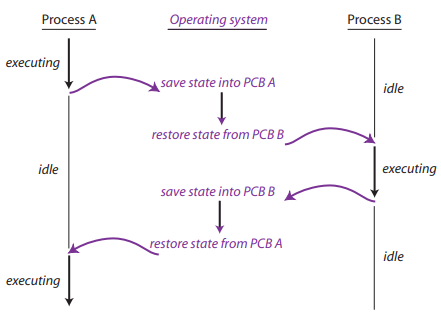
\includegraphics[scale=0.5]{context_switching}
\end{center}
\section{What type of problem do we have to solve?}
Key notions of a general problem:
\begin{itemize}
	\item Computation
	\item Resource
	\item Correctness
\end{itemize}
\textbf{Abstraction} - Hiding information, such as to make the problem easier to solve\\
When developing an abstraction of a real world problem, the abstractions must mirror reality sufficiently closely so conclusions are valid for the real world problem\\
\\
A decision problem D consists of:
\begin{itemize}
	\item A set of instances I
	\item A subset $Y\subseteq I$ of yes instances 
\end{itemize}
A \textbf{graph}, G(V,E), has a finite set V of vertices and a set E of pairs of distinct vertices where no edge is repeated.\\
\textbf{Proper Colouring} - Colouring in which any two adjacent vertices are coloured differently.\\
\textbf{Optimal Colouring} - A proper colouring that uses the smallest number of colours\\
\\
\textbf{Four colour theorem} - Every planar graph can be properly coloured using just 4 colours\\
\textbf{Greedy Algorithm} - An algorithm that works through a list "greedily" choosing the best thing to do\\
\textbf{Brute force colouring} - Try all possible colourings to see if it is legal or not\\
\\
A search problem S consists of:
\begin{itemize}
	\item A set of instances I
	\item A set of solutions J
	\item A binary search relation $R\subseteq I\times J$
\end{itemize}
An optimisation problem is defined as:
\begin{itemize}
	\item A set of instances I
	\item For every instance $x\in I$ there is a set of feasible solutions $f(x)$
	\item For every instance $x\in I$ and for every feasible solution $y\in f(x)$ there is a value $v(x,y)\in \mathbb{N}={0,1,2,...}$ giving the measure of the feasibility solution $y$ for the instance $x$
	\item There is a goal which is either min or max
\end{itemize}
\textbf{Independent set} - A set of vertices in a graph where no two are adjacent\\
\textbf{Maximal Independent Set} - Not contained in any other independent set
\section{How do we develop algorithms to solve fundamental problems?}
Selection sort - Constant time complexity $\mathcal{O}(n^2)$\\
Bubble sort - Worst case complexity $\mathcal{O}(n^2)$ best case complexity $\mathcal{O}(n)$
\section{How do we know an algorithm solves a particular problem}
Ways a software bug can arise:
\begin{itemize}
	\item Programming error
	\item Secondary error like a compiler
\end{itemize}
Waterfall model:
\begin{itemize}
	\item \textbf{Requirements phase} - Produce a specification of what a program is supposed to do
	\item \textbf{Design phase} - Compose a plan for the solution involving Algorithms, Data Structures etc
	\item \textbf{Implementation phase} - Write the code
	\item \textbf{Verification phase} - Test and debug
	\item \textbf{Maintenance} - Continual modification/updating
\end{itemize}
\textbf{Formal Methods} - Mathematically based techniques for the formal specification and verification of software and hardware systems\\
\textbf{Software Testing} - Evaluating an attribute or capability of a program or system and determine that it meets its required results\\
\textbf{Software Metric} - A measure of testing\\
\textbf{Totally Correct} - Correct with respect to some specification and terminates on every input\\
\textbf{Partially Correct} - Only correct with respect to the specification\\
Fundamental aspects of a successful proof of total correctness when using invariants
\begin{itemize}
	\item Initialisation - Show that the invariant holds prior to the first iteration of the loop
	\item Maintenance - Show that the invariant is maintained
	\item Termination - Show that the invariant holds when the loop stops
\end{itemize}
\textbf{Formal Specification} - The study of the specification of a program's properties using a specification language defined by logic\\
\textbf{Formal Verification} - Mathematical techniques used to ensure that a design conforms to some precisely expressed notion of functional correctness
\section{How can we measure how good an algorithm is?}
Resources to measure about an algorithm:
\begin{itemize}
	\item Time
	\item Memory
\end{itemize}
$f=\mathcal{O}(g)$ if there exists $n_0\in \mathbb{N}$ and $k\in Q$ such that $f(n)\leqslant k\cdot g(n)$ whenever $n\geqslant n_0$\\
$f=\Omega(g)$ if there exists $n_0\in \mathbb{N}$ and $k\in Q$ such that $g(n)\leqslant k\cdot f(n)$ whenever $n\geqslant n_0$\\
$f=\Theta(g)$ if $f=\mathcal{O}(g)$ and $f=\Omega(g)$
\section{What exactly is a hard problem?}
\textbf{Tractable} - Can be solved by an algorithm of time complexity $\mathcal{O}(n^k)$\\
\textbf{Efficiently checkable} - Given a potential witness that some instance is a yes-instance, we can check in polynomial time whether the witness is indeed a witness\\
\textbf{Non deterministic algorithm} - An algorithm which guesses the solution, then checks if it's correct
\textbf{P} - The complexity class of efficiently solvable problems\\
\textbf{NP} - The complexity class of efficiently checkable problems\\
\\
A polynomial time transformation from X to Y is an algorithm $\alpha$ that:
\begin{itemize}
	\item Takes an instance I of X as input and provides an instance $\alpha(I)$ of Y as output
	\item Is such that an instance I of X is a yes-instance iff the instance $\alpha(I)$ of Y is a yes-instance
\end{itemize}
\textbf{Cook's theorem} - P=NP iff $SAT\in P$
\end{document}